\chapter{Корзины и мячи}
\label{ch:BucketsAndBalls}

\marginnote{Глава основана на статье \cite{bucketsAndBalls}}

Понятие <<связанные данные>> (Linked Data) по-прежнему недопонято и недооценено. Возможно, эти данные кажутся слишком сложными. 
Попробуем разобраться. Начнём с переменных.

\begin{marginfigure}[0cm]
	{
		\setlength{\fboxsep}{0pt}%
		\setlength{\fboxrule}{1pt}%
		\fcolorbox{gray}{gray}{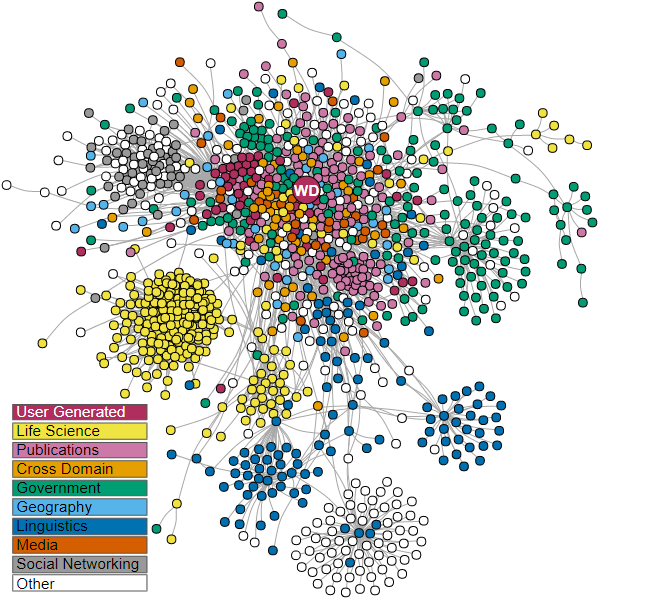
\includegraphics{./intro/bucketsAndBalls/Wikidata_in_linked_open_data.png}}
	}
    \caption[Викиданные в связанном облаке открытых данных]{Викиданные в связанном облаке открытых данных. Базы данных обозначены кружками (Викиданные обозначены как \textit{WD}) с серыми линиями, связывающими базы данных в сети, если их данные выровнены. См. статью в Английской Википедии: \href{https://en.wikipedia.org/wiki/Linked_data}{Linked data}. Wikimedia Commons / \href{https://commons.wikimedia.org/wiki/File:Wikidata_in_the_Linked_Open_Data_cloud_2020-08-20.svg}{Thomas Shafee}}
	\label{fig:Wikidata_in_linked_open_data}
\end{marginfigure}

Что такое переменная в SPARQL? Пусть это будет то, что нужно чем-то заполнить. Но как себе представить это <<то>>? Что-то абстрактное легче представить, если связать с чем-то физическим и конкретным. Трудно представить себе время, но как только мы представим себе часы со стрелками, становится легче. Мы не можем представить себе мебель вообще, но представить стул может каждый.

Другая трудность заключается в том, чтобы сформулировать запрос на языке SPARQL. Хотя работа со SPARQL помогает понять, как работает граф знаний\footnote[][12pt]{\index{Информатика!Граф знаний} Граф знаний~--- это база знаний, которая использует графовую структурированную модель данных для интеграции данных. Графы знаний часто используются для хранения взаимосвязанных описаний сущностей — объектов, событий, ситуаций или абстрактных понятий. Далее будет построен граф знаний (рис.~\ref{fig:Graph_pattern_in_basket_and_balls_notation}).}, запрос SPARQL на него не похож. Это как с символами в математике. <<5 не похоже на пять, в то время как ||||| равно пяти>>.

Итак, как решить проблему с определением переменной и формулировкой SPARQL-запроса?

Представим себе каждый SPARQL-запрос в виде графа связанных между собой корзин и мячей.

Пусть, переменные являются чем-то, что нужно заполнить, но сейчас переменная~--- это абстрактное понятие. Нам нужен физический контейнер, чтобы наполнить его вещами. Нам нужны корзины. И вещи похожие на мячи. Итак, давайте представим выполнение запроса как заполнение корзин мячами.

Тогда процесс заполнения графа мячами будет выглядеть как на рис.~\ref{fig:Query_as_filling_buckets_with_balls}. Корзина \textbf{?A} должна быть заполнена теми мячами, которые имеют отношение \textbf{R} к мячу \textbf{B}.

Рисунок будет понятнее, если мы его упростим и нарисуем прямую линию (рис.~\ref{fig:Graph_pattern_in_basket_and_balls_notation}). Это шаблон графа в нотации <<Корзины и мячи>>. Направление отношения R не показано, но оно всегда слева направо.

\newpage
Тогда процесс написания и выполнения SPARQL-запроса будет состоять из шагов:
\begin{enumerate}
    \item Выберите свои корзины (в них вы будете собирать нужные вам мячи).
    \item Составьте свои условия в виде графа корзин и мячей.
    \item Запустите свой запрос, чтобы наполнить корзины мячами.
\end{enumerate}

\begin{marginfigure}[-4cm]
	{
		\setlength{\fboxsep}{0pt}%
		\setlength{\fboxrule}{1pt}%
		\fcolorbox{gray}{gray}{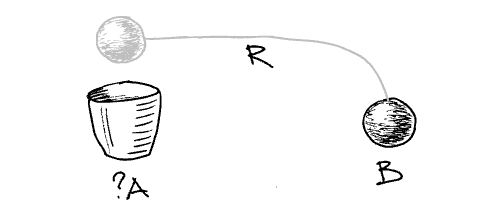
\includegraphics{./intro/bucketsAndBalls/Query_as_filling_buckets_with_balls.PNG}}
	}
    \caption{Образец графа заполнения корзин мячами.}
	\label{fig:Query_as_filling_buckets_with_balls}
\end{marginfigure}

\begin{marginfigure}
	{
		\setlength{\fboxsep}{0pt}%
		\setlength{\fboxrule}{1pt}%
		\fcolorbox{gray}{gray}{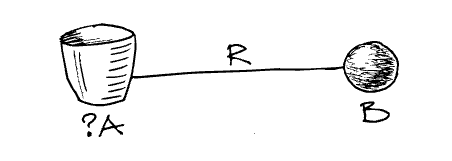
\includegraphics{./intro/bucketsAndBalls/Graph_pattern_in_basket_and_balls_notation.PNG}}
	}
    \caption{Шаблон графа в нотации <<Корзины и мячи>>.}
	\label{fig:Graph_pattern_in_basket_and_balls_notation}
\end{marginfigure}

Теперь напишем запрос, чтобы, например, получить всех руководителей областей России, выполняя такие шаги:

\begin{enumerate}
    \item Возьмём две корзины, одна для регионов и одна для руководителей.
    \item Корзину для регионов привяжем к мячу <<область России>> отношением <<экземпляр>> (instance of). Тогда из множества мячей~--- объектов Викиданных~--- в эту корзину попадут только те мячи, которые являются областью России. Корзина для регионов связана с корзиной <<руководитель>> (head) отношением <<имеет руководителя>>, в нашем случае это будет губернатор или глава области.
\end{enumerate}

Сделаем запрос более интересным и добавим ещё одну корзину для фотографий губернаторов. Вот теперь запрос в нотации <<Корзины и мячи>> будет как на рис.~\ref{fig:Query_in_basket_and_balls_notation}.

\begin{figure*}[h!]
    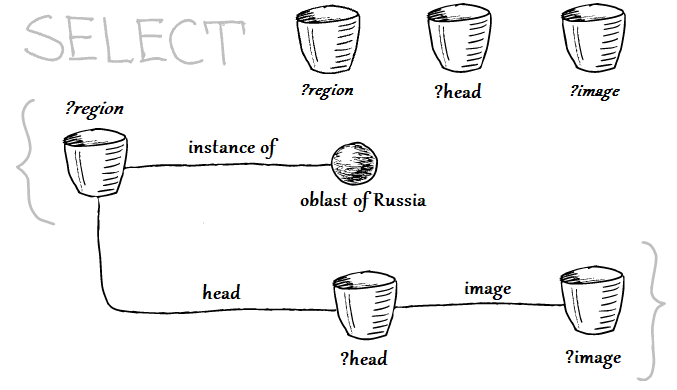
\includegraphics[width=0.7\linewidth]{./intro/bucketsAndBalls/Query_in_basket_and_balls_notation.PNG}
    \caption{Запрос в нотации <<Корзины и мячи>> для заполнения корзин <<регион>> мячами <<область России>>, <<руководитель>>~--- губернаторами или главами области, <<изображение>>~--- их фотографиями.}
	\label{fig:Query_in_basket_and_balls_notation}
\end{figure*}

\newpage
После выполнения запроса (рис.~\ref{fig:Query_in_basket_and_balls_notation}) наши корзины будут выглядеть как на рис.~\ref{fig:3_buckets_region_head_image}.

\begin{marginfigure}
	{
		\setlength{\fboxsep}{0pt}%
		\setlength{\fboxrule}{1pt}%
		\fcolorbox{gray}{gray}{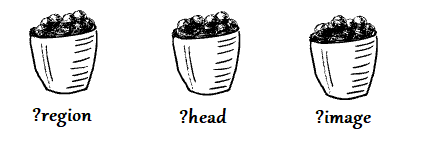
\includegraphics{./intro/bucketsAndBalls/3_buckets_region_head_image.PNG}}
	}
    \caption{Корзины после выполнении запроса на рис.~\ref{fig:Query_in_basket_and_balls_notation}. \textit{?region}~--- это области России, \textit{?head}~--- это руководители, \textit{?image}~--- это фотографии руководства.}
	\label{fig:3_buckets_region_head_image}
\end{marginfigure}

Теперь перейдём в сервис \href{https://query.wikidata.org/}{Wikidata Query Service} 
(далее WDQS\footnote[][15pt]{См. пояснения о службе WDQS на c.~\pageref{sect:WDQS}.})  и напишем этот запрос на языке SPARQL. Сначала выберем и назовём корзины для заполнения так:

\begin{lstlisting}[ language=SPARQL ]
SELECT DISTINCT ?region ?head ?image
\end{lstlisting}

Далее напишем условия соответствия мячей корзинам. Все условия в SPARQL должны заключаться в фигурные скобки, как на рис.~\ref{fig:Query_in_basket_and_balls_notation}.

Когда нам нужно определённое отношение или мяч, нам нужно использовать их идентификаторы. Викиданные облегчают поиск идентификатора и подсказывают его, когда вы выбираете отношение (свойство) или мяч (объект) по его имени (метке). Чтобы указать отношения в графе знаний Викиданных, мы используем префикс \textit{wdt:}, а для объектов (наших мячей)~--- префикс \textit{wd:}.

Следуя нашей нотации (рис.~\ref{fig:Query_in_basket_and_balls_notation}), напишем условия для заполнения первой корзины \textit{?region}, затем напишем первое отношение. Поскольку общей частью идентификаторов прямых отношений является wdt, мы пишем \textit{wdt}:, а затем, в сервисе WDQS, нажимаем Ctrl+пробел, чтобы запустить службу подсказок или  автозаполнения Викиданных (рис.~\ref{fig:WDQS_popup_instance_of}).

\begin{marginfigure}[-2.5cm]
	{
		\setlength{\fboxsep}{0pt}%
		\setlength{\fboxrule}{1pt}%
		\fcolorbox{gray}{gray}{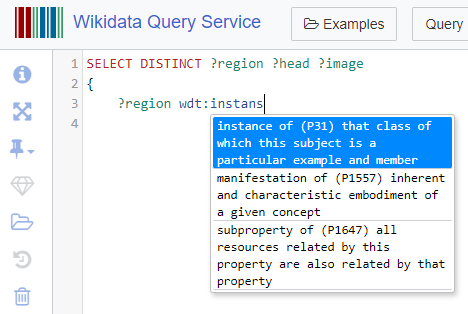
\includegraphics{./intro/bucketsAndBalls/WDQS_popup_instance_of.PNG}}
	}
    \caption{С помощью команды Ctrl+пробел открылось выпадающее контекстное меню автозаполнения свойства Викиданых.}
	\label{fig:WDQS_popup_instance_of}
\end{marginfigure}

После этого мы воспроизведём модель из рис.~\ref{fig:Query_in_basket_and_balls_notation} в реальном запросе SPARQL.

Обычно при написании SPARQL-запроса его представляют в виде таблицы с тремя столбцами: субъект, предикат, объект или на языке Викиданных~--- объект, свойство, значение.

Возможно, начинающему программисту осваивать язык SPARQL будет проще, если хотя бы ваши первые запросы будут напоминать граф. Попробуем взять граф на рис.~\ref{fig:Query_in_basket_and_balls_notation} и написать максимально похожим образом SPARQL-запрос (листинг~\ref{lst:linkRegionsOfHeads}).

\begin{lstlisting}[ language=SPARQL, caption={\href{https://w.wiki/4NVc}{Список руководителей областей России с фотографиями}\protect\footnotemark},label=lst:linkRegionsOfHeads, ]
SELECT DISTINCT ?region ?head ?image
{
    ?region wdt:P31 wd:Q835714; # oblast of Russia
            wdt:P6  ?head. # heads of government
    ?head  wdt:P18 ?image. # images of heads of government
}
\end{lstlisting}
\footnotetext{Получено 44 ссылки на области России и их глав правительства. Ссылка на SPARQL-запрос: \href{https://w.wiki/4NVc}{https://w.wiki/4NVc}}

\newpage Теперь посмотрите, как этот запрос выглядит в сервисе WDQS, и запустите его. Затем нажмите на значок глаза слева и выберите \textit{``image grid``} (рис.~\ref{fig:WDQS_drop_down_result_type}), чтобы просмотреть результаты в виде сетки изображений.

\begin{marginfigure}
	{
		\setlength{\fboxsep}{0pt}%
		\setlength{\fboxrule}{1pt}%
		\fcolorbox{gray}{gray}{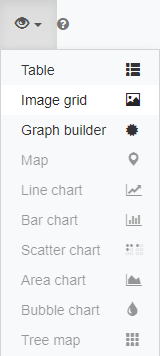
\includegraphics[width=0.5\linewidth]{./intro/bucketsAndBalls/WDQS_drop_down_result_type.PNG}}
	}
    \caption{Выбор отображения результатов в виде \textit{``image grid``} (сетки изображений).}
	\label{fig:WDQS_drop_down_result_type}
\end{marginfigure}

Это неплохо для первого результата, но теперь под каждой фотографией мы видим только идентификаторы людей и областей. Если мы щёлкнем по гиперссылке идентификатора, мы получим много информации об этом объекте. Но было бы нагляднее кроме идентификаторов указать имена людей и названия областей (меток) в результате запроса. Это похоже на наклеивание этикеток на наши корзины (рис.~\ref{fig:Query_in_basket_and_balls_notation_with_ids}).

\begin{figure*}[h!]
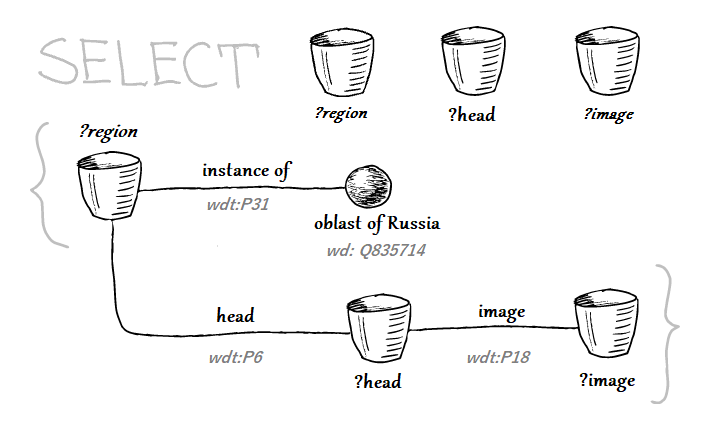
\includegraphics[width=0.6\linewidth]{./intro/bucketsAndBalls/Query_in_basket_and_balls_notation_with_ids.png}
\caption{Запрос в нотации <<Корзины и мячи>> с номерами свойств и объектов Викиданных.}
\label{fig:Query_in_basket_and_balls_notation_with_ids}
\end{figure*}

Метка(\textit{``Label``})~--- это то, что есть у каждого мяча, то есть объекта Викиданных. Метка – это имя, позволяющее различать объекты между собой. В Викиданных есть сервис, упрощающий вывод меток по запросу. Для этого достаточно добавить в конец имени переменной слово \textit{``Label``} и вызвать нужный сервис. Чтобы вызвать этот сервис, на новой строке внутри фигурных скобок наберите Ctrl + пробел и когда вы начнёте писать слово \textit{``Label``}, тогда будет добавлена строка с этим сервисом\footnote[][12pt]{Пример вызова этого сервиса представлен в листинге~\ref{lst:regionsOfHeads}, в строке 8. В этой строке, языком для меток, указан русский язык (код ``ru``)}. По умолчанию вы получаете подсказку с языком интерфейса и английским языком в качестве альтернативы, если метка недоступна на языке выбранного интерфейса Викиданных.

Викиданные полны таких замечательных сервисов, и для окончательного запроса мы воспользуемся ещё одним. Чтобы получить результат сразу в виде набора фотографий глав областей, без дополнительного нажатия на значок глаза, поместите где-нибудь в своём запросе следующую конструкцию для WDQS:
\begin{lstlisting}[ language=SPARQL ]
#defaultView:ImageGrid
\end{lstlisting}

На самом деле не всё нужно писать вручную. Когда вы начнёте печатать, сервис автозаполнения предложит варианты.

Наш последний запрос представлен на листинге~\ref{lst:regionsOfHeads}. Фрагмент результата его выполнения показан на рис.~\ref{fig:Result_of_the_request}.

\lstset{numbers=left, firstnumber=1, frame=single}
\begin{lstlisting}[ language=SPARQL, caption={\href{https://w.wiki/4ENR}{Список глав областей России}\protect\footnotemark}, label=lst:regionsOfHeads, ]
# List of regions of the Russia and images of heads of government
#defaultView:ImageGrid
SELECT DISTINCT ?region ?regionLabel ?head ?headLabel ?image
{
  ?region wdt:P31 wd:Q835714; # ?region is Oblast of Russia
          wdt:P6  ?head.      #         has head of government
  ?head  wdt:P18 ?image.      # head has image
  SERVICE wikibase:label {bd:serviceParam wikibase:language "ru"} 
}
\end{lstlisting}

\footnotetext{Получено 44 области России и их руководителей. Ссылка на SPARQL-запрос: \href{https://w.wiki/4ENR}{https://w.wiki/4ENR}}

\begin{figure*}[h!]
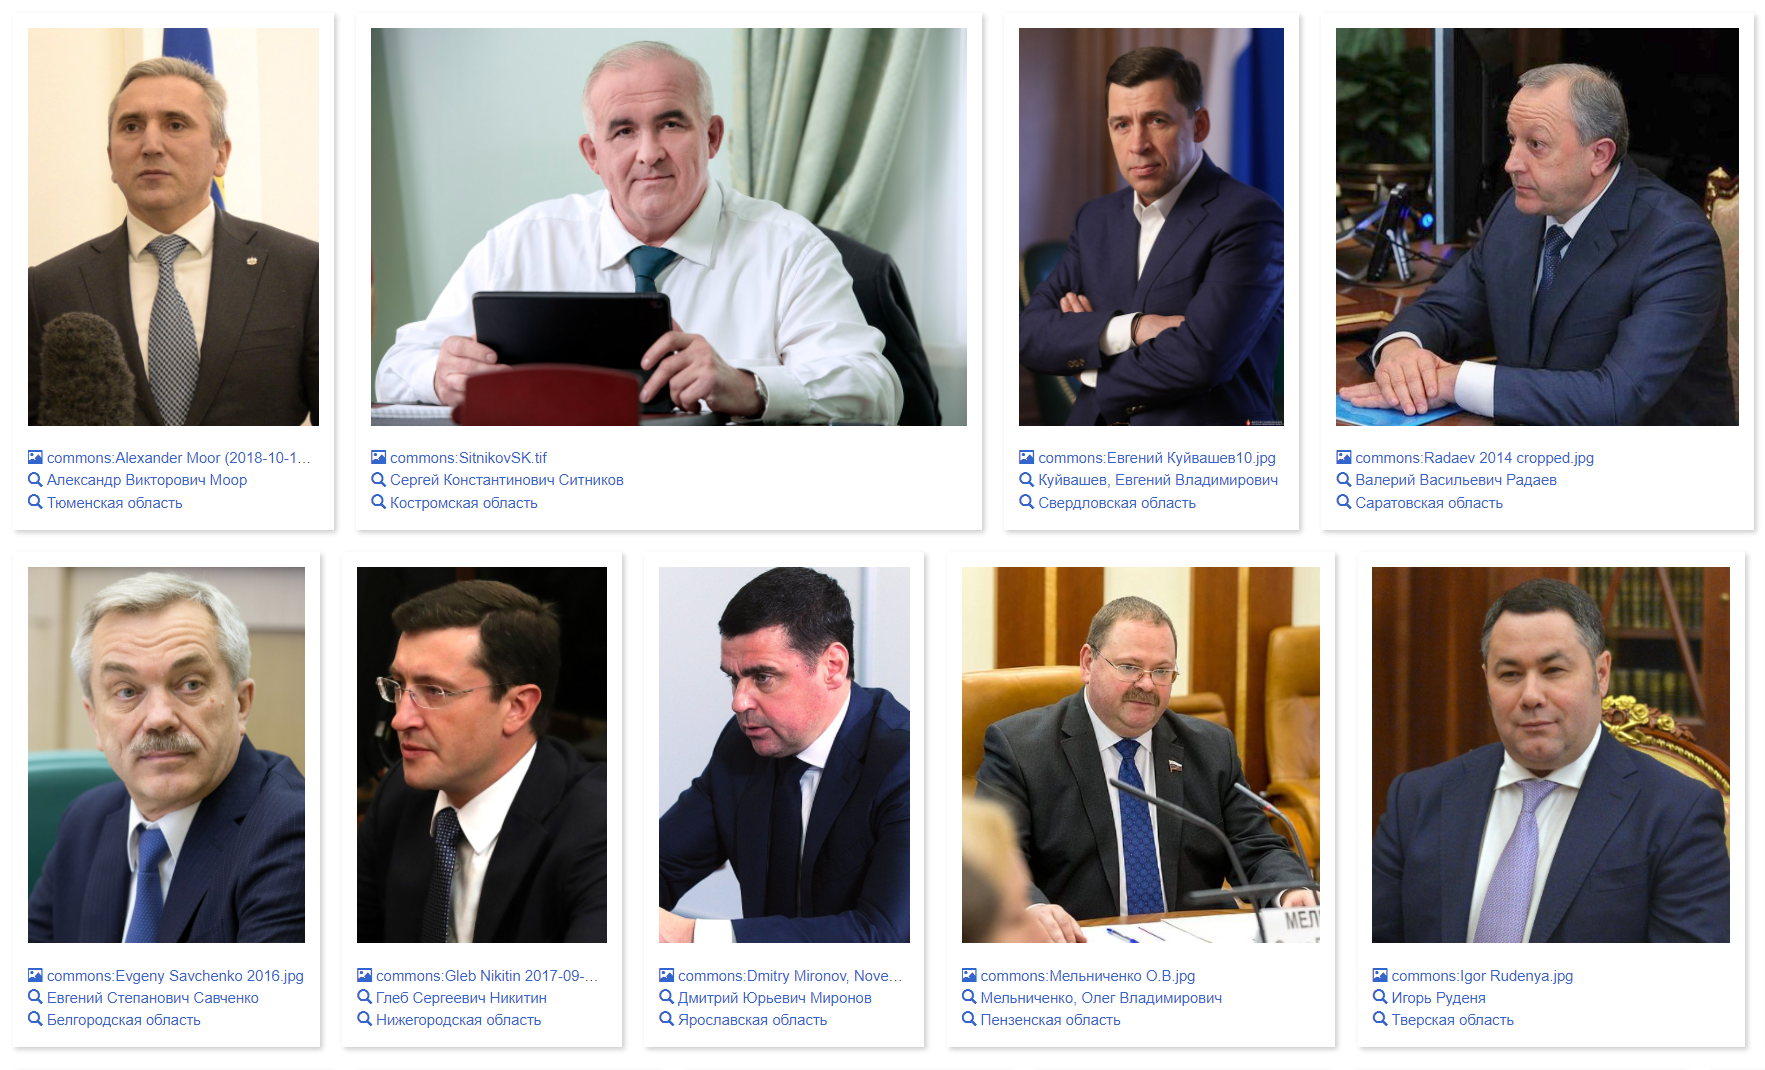
\includegraphics[width=0.6\linewidth]{./intro/bucketsAndBalls/result_of_request_for_photos_of_heads_of_government.png}
\caption{Результат запроса в виде сетки изображений.}
\label{fig:Result_of_the_request}
\end{figure*}


Такое представление о запросах SPARQL, как о связанных корзинах и мячах, может быть полезным, по крайней мере, в начале освоения Викиданных. И, конечно, у каждой метафоры есть свои ограничения. Например, нельзя поместить один и тот же мяч в две разные настоящие корзины, но в эти виртуальные~--- можно. <<Корзины и мячи>> могут быть полезны, чтобы вскарабкаться на высоту абстракции Викиданных.
